

Bluetooth est l'un des protocoles les plus utilisés pour réaliser des communications à courtes distances. Il implémente plusieurs mécanismes afin de chiffrer l'échange de données entre deux dispositifs.\\


\textbf{Note} : La section de ce rapport n'a pas pour objectif de traiter la cryptographie même du protocole Bluetooth, ni la manière dont les clés sont générées algorithmiquement. Pour des informations complémentaires sur la génération des clés, il est proposé de lire deux articles. Le premier est élaboré par l'instance officielle du Bluetooth et le deuxième est un \textit{whitepaper} rédigé par le très célèbre fabricant d'appareils de mesures électroniques Teledyne Lecroy : 
\begin{center}
    \footnotesize{\url{http://blog.bluetooth.com/bluetooth-pairing-part-1-pairing-feature-exchange}}
    \footnotesize{\url{http://www.fte.com/webhelp/sodera/Content/Documentation/WhitePapers/BTLE/BluetoothSmartSecurity.htm}}
\end{center}


La sécurité de la technologie Bluetooth a évolué au fil des diverses versions. Actuellement, les versions 4.2 et 5.0 ont les mêmes caractéristiques. Aucun élément de sécurité supplémentaire n'a été ajouté dans le Bluetooth 5.0 \cite{WhatsNe89:online}. Cependant, beaucoup de changements sont survenus entre les versions 4.0, 4.1 et 4.2. Ces anciennes versions ne seront pas abordées en détail, puisque presque aucun dispositif Bluetooth moderne n'est distribué sans le support de la version 4.2 au minimum. \\

Lors de l'explication des différents blocs de la couche \textit{Host} du Bluetooth, le bloc \texttt{Security Manager} a été abordé (cf. \cref{sec-protocols_BLE_security_manager}). Ce bloc s'occupe des générations et des sauvegardes de clés, de même que des méthodes et protocoles utilisés pour appairer deux dispositifs et partager les clés de connexion.\\

Lors de la mise en place d'une connexion sécurisée BLE, deux définitions sont utilisées :
\begin{itemize}
    \item Initiateur (\textit{initiator}) : correspond au maitre au niveau de la couche \texttt{Link Layer} et est aussi appelé centrale pour la couche GAP.
    \item Répondeur (\textit{responder}) : correspond à l'esclave au niveau de la couche \texttt{Link Layer} et est aussi appelé périphérique pour la couche GAP.
\end{itemize}

\subsection{Modes et niveaux de sécurité}
Dans la \cref{sec-protocols_BLE_GAP}, le bloc GAP a été défini comme étant l'élément s'occupant de l'authentification des centrales qui souhaitent se connecter auprès du périphérique. 
Il existe le concept de modes et niveaux de sécurité pour une connexion BLE. Voici la définition de ceux-ci :
\begin{enumerate}
    \item Mode 1 :
    \begin{enumerate}
        \item Niveau 1: Pas de sécurité (ni authentifiée, ni chiffrée);
        \item Niveau 2: Appairage non authentifié avec transfert de données chiffrées;
        \item Niveau 3: Appairage authentifié avec transfert de données chiffrées;
        \item Niveau 4: Appairage authentifié avec \textit{LE Secure Connections} et transfert de données chiffrées.
    \end{enumerate}
    \item Mode 2 :
    \begin{enumerate}
        \item Niveau 1: Appairage non authentifié avec transfert de données signées;
        \item Niveau 2: Appairage authentifié avec transfert de données signées.
    \end{enumerate}
\end{enumerate}


Toutes les connexions commencent en \textbf{mode 1} et \textbf{niveau 1} \cite{microchip_ble_security:online}. 

\subsection{Appairage et attachement}

L'appairage Bluetooth (\textit{pairing} en Anglais) est le processus qui définit l'échange des données de sécurité et la génération des clés \cite{BLEpairi85:online}\cite{Bluetoot72:online}.  Il y a au total trois phases lors de ce processus d'appairage, lesquelles sont visibles sur la \cref{fig-pairing-flowchart} et expliquées en détail dans les sous-sections qui suivent. 

\begin{figure}[ht!]
    \centering
    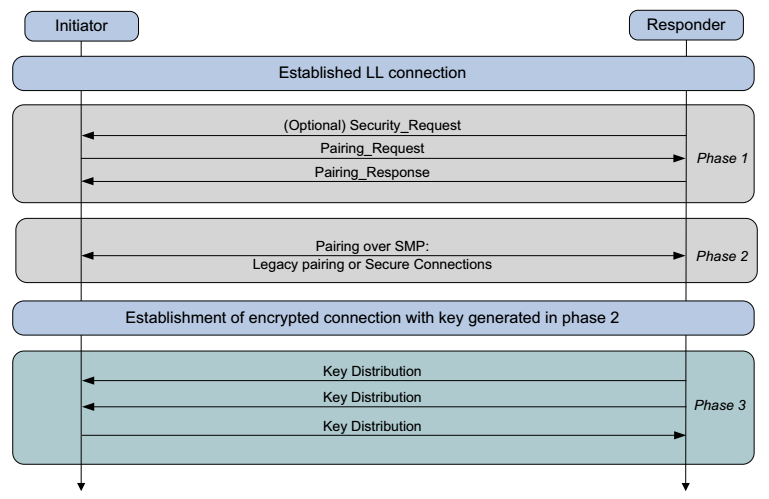
\includegraphics[width=1.0\textwidth]{Figures/Security/BLE/pairing-flowchart.png}
    \caption{Diagramme du processus d'appairage}
    \label{fig-pairing-flowchart}
\end{figure}

Ce processus de sécurité n'est pas forcément déclenché directement à la connexion, car plusieurs niveaux de sécurité peuvent être appliqués pour différents attributs. Par exemple, si une périphérique souhaite uniquement protéger un seul et unique attribut, il peut placer tous les autres attributs en Mode 1 Niveau 1. Le processus d'appairage ne sera déclenché que lorsque un attribut du mode 1 niveau 2 (au minimum) est accédé. L'appairage consiste à l'authentification de l'identité entre deux dispositifs et la création d'un canal chiffré utilisant une \textit{Short-Term Key} (STK). Une fois ce canal, créé, il faut ensuite distribuer des \textit{Long-Term Keys} (LTK), c'est à la fin de cette que la connexion est considéré comme attachée (\textit{bonded}). Les LTK seront ensuite sauvegardées sur les deux dispositifs pour chiffrer les futures communications sans nécessiter un nouvel appairage. \\

Il est important de comprendre le fonctionnement de ce processus, car tous ces modes doivent être configurés manuellement sur un microcontrôleur. 


\subsubsection{Phase 1: \textit{Pairing Feature Exchange}}

% TODO : 
% Cette phase a pour but d'échanger les informations sur les 
    
    
La phase 1 a pour objectif de partager les prérequis qui sont exigés pour la connexion.
Parmi ces données, on trouve diverses informations, telles que les entrées/sorties disponibles sur le périphérique, si l'utilisateur exige une protection \textit{man-in-the-middle} (MITM), etc. Ceux-ci seront ensuite analysés en phase 2 afin de s'assurer que le mode et niveau choisi pour la connexion est possible avec les informations fournies dans la phase 1. Les dispositifs doivent indiquer les capabilités de leurs I/O à l'aide des types définis sur la \cref{fig-io_capabilities} pour les entrées et \cref{fig-output_capabilities} pour les sorties.

\begin{figure}[ht!]
    \centering
    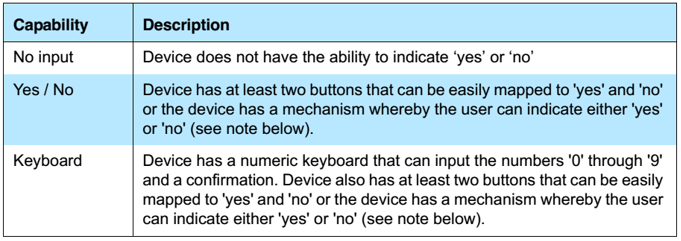
\includegraphics[width=0.85\textwidth]{Figures/Security/BLE/io_capabilities.png}
    \caption{Capacité des entrées disponibles sur un dispositif Bluetooth}
    \label{fig-io_capabilities}
\end{figure}

\begin{figure}[ht!]
    \centering
    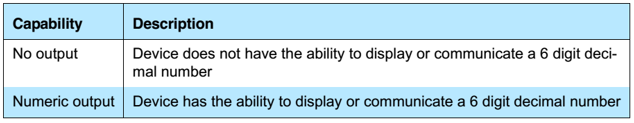
\includegraphics[width=0.85\textwidth]{Figures/Security/BLE/output_capabilities.png}
    \caption{Capacité des sorties disponibles sur un dispositif Bluetooth}
    \label{fig-output_capabilities}
\end{figure}



%OOB, or Out-of-Band, uses an external means of communication to exchange some information used in the pairing process. The OOB media could be any other wireless communication standard which can carry the corresponding information for pairing, like NFC or QRCode.

    
\subsubsection{Phase 2 : \textit{LE Legacy Pairing} ou \textit{LE Secure Connections}}


%After pairing feature exchange, initiator and responder should determine what key generation method will be used. Here is sample C syntax coding for the key generation method:

Après l'échange des \textit{pairing features} de la phase 1, la centrale et le périphérique doivent s'accorder sur quelle méthode utiliser pour l'échange et la génération des clés. \\



Depuis l'introduction du Bluetooth 4.2, si les deux dispositifs sont compatibles avec l'option LE Secure Connections et Secure Simple Pairing (SSP), alors il est conseillé d'utiliser ceux-ci (mode 1 niveau 4). La nouveauté majeure dans ce type de connexion est l'algorithme utilisé pour la génération des clés. Celui-ci est maintenant basé sur un échange et génération de clés publiques à l'aide de l'algorithme \textit{Elliptic Curve Diffie Hellman}\footnote{\url{https://en.wikipedia.org/wiki/Elliptic-curve_Diffie\%E2\%80\%93Hellman}} (ECDH) \cite{ble_basic_intro:online}. La \cref{fig-algorithms_4_2} illustre la différence entre le mode \textit{Legacy} (avant BLE 4.2) et les nouveaux algorithmes utilisés pour l'appairage et le \textit{bonding} \cite{Differen40:online}. \\


\begin{figure}[ht!]
    \centering
    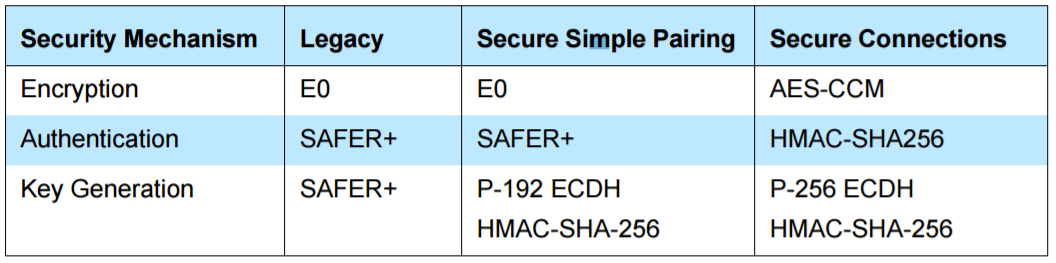
\includegraphics[width=0.85\textwidth]{Figures/Security/BLE/algorithms_4_2.PNG}
    \caption{Comparaison des algorithmes de générations de clés en fonction des versions BLE}
    \label{fig-algorithms_4_2}
\end{figure}



En Bluetooth Low Energy, il existe quatre méthodes pour la génération et l'échange de clés, de même que l'authentification de l'utilisateur: 

\begin{itemize}
    \item \texttt{\textit{\textbf{Just Works}}} : la STK est générée sur les deux dispositifs et est envoyée en \textit{plain-text}. Une fois ces clés publiques échangées, le \textit{responder} génère un \textit{nonce} aléatoire avec lequel il génère une valeur de confirmation nommée \texttt{Cb}. Ces deux paramètres (nonce et Cb) sont ensuite transmis à l'initiateur. En parallèle, l'initiateur génère son propre \textit{nonce} et le transfert au \textit{responder}. L'initiateur utilise ensuite le \textit{nonce} reçu de la part du \textit{responder} pour générer la valeur de confirmation nommée \texttt{Ca}. Les valeurs \texttt{Cb} et \texttt{Ca} doivent être identiques, si c'est le cas, la connexion est acceptée\cite{ble_basic_intro:online}.
    Cette méthode ne fournit pas d'opportunité à l'utilisateur de vérifier la légitimité du périphérique connecté. Une attaque de type \textit{man-in-the-middle} peut toujours prendre place\cite{microchip_ble_security:online}.
    
% The STK is generated on both sides, based on the packets exchanged in plain text. This method provides no security against man-in-the-middle (MITM) attacks.

% Once the devices exchange their public keys, the non-initiating device will generate a nonce, which is essentially a random seed value, and then use it to generate a confirmation value Cb. It then sends the Cb along with the nonce to the initiating device. At the same time, the initiating device generates its own nonce and sends it to the non-initiating device. The initiating device then uses the non-initiating device’s nonce to generate its own confirmation value Ca which should match Cb. If the confirmation values match, then the connection proceeds.

% By virtue of the ECDH key exchange, the Just WorksTM pairing method in LE Secure Connections has substantially more resilience to passive eavesdropping compared to the same method in LE Legacy Connections. However, since this method does not give the user a way to verify the authenticity of the connection, it is still vulnerable to MITM attacks.

    \item \texttt{\textit{\textbf{Passkey Display}}} : un des deux dispositifs affiche un code PIN (\textit{passkey}) de minimum 6 digits (en LE Secure Connection) et de préférence aléatoire. Le deuxième dispositif doit demander à l'utilisateur d'entrer le code affiché. Cette méthode Il faut donc au minimum un clavier sur un périphérique et un écran sur l'autre. Une protection \textit{man-in-the-middle} est prodigué, sauf si le PIN généré est à la vue de tous.
  
%   Passkey Display
% One of the peers displays a randomly generated 6-digit passkey and the other side as asked to enter it. In certain cases both sides enter the key, if no display is available. This method provides protection against MITM attacks.
    
    \item \texttt{\textit{\textbf{Out Of the Band (OOB)}}} : lors de la phase 1, les deux dispositifs indiquent s'ils acceptent un échange de clé par OOB. Cela signifie que l'échange de clés ne s'effectue pas à l'aide de la bande de fréquence du Bluetooth (2.4 GHz), mais à l'aide d'un autre mécanisme. Les méthodes les plus connues sont l'échange par communication NFC ou la lecture d'un QR code. \cite{microchip_ble_security:online} \cite{ble_basic_intro:online}.
    
%     Out of Band (OOB)
% This method has the additional data transferred by means other than the BLE radio (such as another wireless technology like NFC). This method also provides protection against MITM attacks.
    
    \item \texttt{\textit{\textbf{Numeric Comparison}}} : cette méthode utilise la même procédure que \texttt{Just Works}, mais rajoute une nouvelle étape à la fin. Une fois que les périphériques confirment la réception des \textit{nonces} utilisés pour la génération des clés, ils génèrent un nombre aléatoire avec ceux-ci. Les deux périphériques doivent ensuite l'afficher et si l'utilisateur voit que les deux valeurs sont identiques, alors il doit appuyer sur un bouton \textit{OK} pour valider que les deux périphériques soient bien authentifiés entre eux. Si ce n'est pas un cas, un bouton \textit{NOT OK} doit être pressé. \\
    
% Numeric Comparison (also called LE Secure Connections Pairing in BLE v4.2)
% This method uses an algorithm called Elliptic curve Diffie–Hellman (ECDH) for key generation, and a new pairing procedure for the key exchange.
% This pairing method follows the exact same procedure as the Just WorksTM pairing method, but adds another step at the end. Once the devices confirm that the confirmation values match, then both devices will independently generate a final 6 digit confirmation value using both of the nonces. They both then display their calculated values to the user. The user then manually checks that both values match and ok’s the connection. This extra step allows this pairing method to provide protection from MITM attacks.
\end{itemize}

Le choix de la méthode utilisée dépend ensuite des paramètres échangés à l'aide du \textit{pairing request} et \textit{pairing response}. Si l'option OOB est possible pour les deux périphériques, elle sera activée par défaut. Le reste des méthodes est choisi en fonction du tableau affiché sur la \cref{fig-ble_choose_security}. L'un des algorithmes présentés est ensuite choisi à la suite des paramètres échangé précédemment. \\


\begin{figure}[ht!]
    \centering
    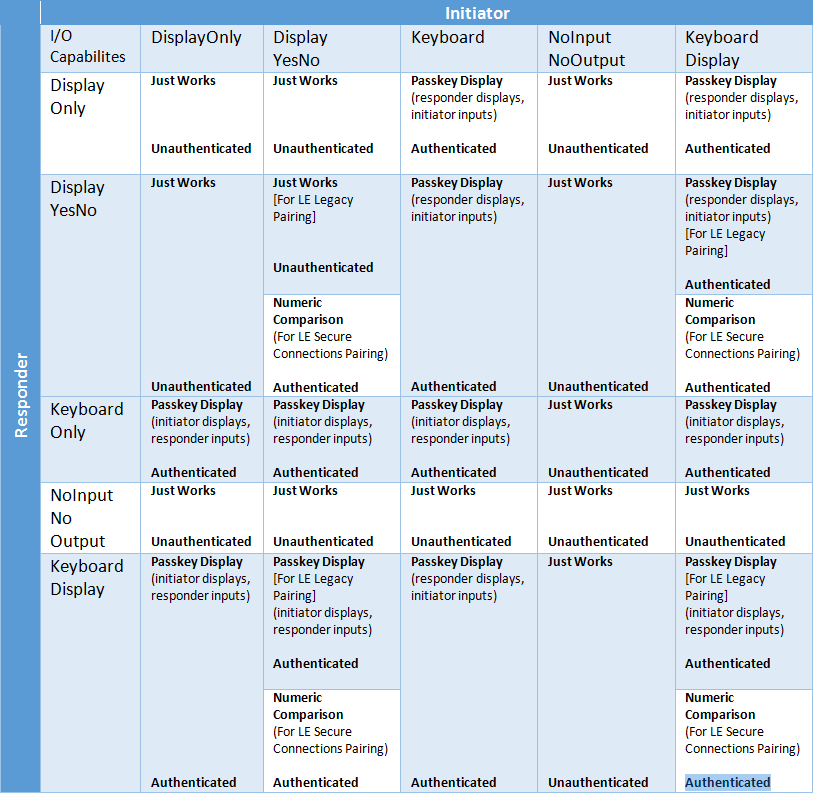
\includegraphics[width=1.0\textwidth]{Figures/Security/BLE/ble_choose_security.png}
    \caption{Choix de la méthode de sécurité en fonction des entrées/sorties}
    \label{fig-ble_choose_security}
\end{figure}

Dans le cas d'un smartphone, celui-ci dispose à la fois d'un clavier et d'un écran. Il offre donc le niveau de sécurité maximal pour l'échange d'informations à l'aide du Bluetooth. 
Le tableau de la \cref{fig-ble_choose_security} représente les recommandations pour les méthodes à utiliser, mais cela n'empêche pas le développeur de mettre en place, par exemple, un \textit{passkey} sans avoir d'écran sur le \textit{responder}. C'est l'une des raisons pour lesquelles beaucoup de périphériques dans le commerce utilisent des \textit{passkeys} tels que 0000 ou 1234 pour la première connexion. Pour cela, les périphériques sont obligés de mentir lorsqu'il envoie le paquet de réponses à l'initiateur. Ils indiquent qu'ils sont de type \textit{\textbf{display only}} alors que cette information est fausse. L'initiateur, la plupart du temps un smartphone ou ordinateur, choisi à l'aide du tableau la méthode qu'il doit appliqué et choisi \textit{initiator} : \textit{Keyboard} + \textit{Display} et \textit{responder} : \textit{display only}. Le smartphone demande ainsi à l'utilisateur d'enter le \textit{passkey}. 
Ce type d'approche détruit le concept d'authentification, car le but initial du \textit{passkey} est de s'assurer que la personne qui se connecte est bien celle qui est en face du périphérique, et donc qui a un accès physique à ce dernier avec la visibilité du \textit{passkey} sur l'écran. \\

Dans le cadre de ce projet, c'est le choix du \textit{passkey} qui a été retenu. Un \textit{passkey} aléatoire est présent dans chaque DevBox et est uniquement accessible à une personne de confiance (cf. \cref{sec-smartcanton_devbox_security} pour plus de détail sur l'implémentation). Mais le PIN n'est pas connu à l'avance, contrairement à la plupart des périphériques du marché où celui-ci est identique sur tous les périphériques vendus.\\




\subsubsection{Phase 3 : \textit{Transport Specific Key Distribution}}

Aussitôt que l'authentification est réussie, les deux dispositifs génèrent une Long Term Key (LTK) qui sera utilisée pour le chiffrement des futures connexions \cite{Bluetoot97:online}. Toutes les prochaines reconnexions des périphériques utiliseront cette clé, sans avoir besoin de réitérer les deux phases précédentes.




%-------------------------------------------------------------------------------------
\subsection{Recommandations de sécurité}
\label{sec-security_ble_recommendatiions}

En mai 2017, le National Institute of Standards and Technology (NIST) a publié un document intitulé \textit{Guide to Bluetooth Security}. Dans ce document de 67 pages, le NIST explique les vulnérabilités présentes sur des dispositifs Bluetooth, ainsi que les différentes failles qui peuvent y être associées \cite{GuidetoB8:online}. Le document analyse la sécurité de tous les protocoles Bluetooth récents (Low Energy ou \textit{Standard}). Il explique en outre les concepts de cryptographie qui sont utilisés pour la génération des clés. Voici le lien de la publication : 
\begin{center}
    \small{\url{http://nvlpubs.nist.gov/nistpubs/SpecialPublications/NIST.SP.800-121r2.pdf}}
\end{center}

À la fin dudit document, 37 recommandations sont proposées pour optimiser la sécurité sur un système utilisant le Bluetooth. Voici quatre exemples de recommandations extrêmement pertinentes pour le projet. La première indique le mode et le niveau de sécurité devant être utilisés sur les périphériques : 

\begin{quote}
\begin{center}
    \textit{"15. Bluetooth 4.2 devices and services using low energy functionality should use Security Mode 1 Level 4 whenever possible. Low energy Security Mode 1 Level 4 implements Secure Connections mode and provides the highest security available for 4.2 low energy devices. If Security Mode 1 Level 4 is not available, recommend using Security Mode 1 Level 3 instead"}
\end{center}
\end{quote}

Le KW41Z supporte tous les modes de sécurité et niveaux de sécurité. Cette recommandation peut ainsi être utilisée dans le projet.\\


Dans ce projet, un certain nombre de profils Bluetooth devant être implémentés, il est important de connaitre les recommandations y relatives. Voici la seule proposée pour les profils et services Bluetooth Low Energy dans le document : 

\begin{quote}
\begin{center}
    \textit{"17. Unneeded and unapproved service and profiles should be disabled. Many Bluetooth stacks are designed to support multiple profiles and associated services. The Bluetooth stack on a device should be locked down to ensure only required and approved profiles and services are available for use"}
\end{center}
\end{quote}

Par défaut, beaucoup de profils Bluetooth sont activés sur un même périphérique. Cependant, si l'utilisateur final n'a pas d'utilité à tous ces services, il convient de les désactiver afin qu'une éventuelle faille ne puisse être exploitée. Il est ici fait référence à des \textit{unapproved services}, référence qui peut être interprétée de deux façons. En premier lieu, il pourrait s'agir des services standards Bluetooth et fournis par la spécification Bluetooth. Néanmoins, cela semble beaucoup trop restrictif comme approche. Si un programmeur ne peut pas développer son propre service, il lui est impossible de faire certaines applications, car elles n'ont pas toutes été prévues par la spécification. L'on pourrait considérer, en second lieu, qu'aucun service non autorisé au sein du développement de l'application (par exemple un service de débogage) ne devrait être intégré dans le produit final. La seconde interprétation parait plus sensée avec les besoins des développeurs et des applications.\\

Lorsqu'une entreprise ou entité dispose de plusieurs périphériques Bluetooth Low Energy, il est important de garder une trace de ceux-ci, de sorte à créer une \textit{whitelist}. C'est pour cela que le NIST adresse la recommandation suivante :

 \begin{quote}
\begin{center}
    \textit{"6. Maintain a complete inventory of all Bluetooth-enabled wireless devices and addresses (BD\_ADDRs)."}
\end{center}
\end{quote}


Les dispositifs sont bien souvent protégés par des codes PIN, afin de ne pas autoriser n'importe quelle centrale à s'appairer avec celui-ci. NIST propose les recommandations suivantes pour la génération de ces codes PIN :
\begin{quote}
\begin{center}
    \textit{"9. Choose PIN codes that are sufficiently random, long and private. Avoid static and weak PINs, such as all zeroes. PIN codes should be random so that malicious users cannot easily guess them. Longer PIN codes are more resistant to brute force attacks. For Bluetooth 2.0 (or earlier) devices, an eight-character alphanumeric PIN should be used, if possible. The use of a fixed PIN is not acceptable."}
\end{center}
\end{quote}

Toutes ces recommandations sont parfois difficiles, voire impossibles à implémenter selon le type d'équipement utilisé. Si l'équipement le permet, il est toutefois préférable de les appliquer.

